\documentclass[10pt]{article}
\usepackage[a3paper,landscape,margin=1.6cm]{geometry}
\usepackage[scaled]{helvet}
\renewcommand\familydefault{\sfdefault}
\usepackage[T1]{fontenc}
\usepackage{amsmath,amssymb,xcolor,tikz,pgfplots,booktabs,array,adjustbox}
\usetikzlibrary{positioning,arrows.meta,fit,backgrounds,calc,shapes.misc}
\pgfplotsset{compat=1.16}
\pagestyle{empty}
\setlength{\parindent}{0pt}
\newcommand{\nsamples}{16{,}500}
\newcommand{\nchanges}{10}


% ---------- palette ----------
\definecolor{layerfill}{HTML}{FFFBD6}
\definecolor{layerline}{HTML}{BDB76B}
\definecolor{okfill}{HTML}{DDF2E3}
\definecolor{okline}{HTML}{2F7D4F}
\definecolor{todofill}{HTML}{F2F2F2}
\definecolor{todoline}{HTML}{8A8A8A}
\definecolor{busfill}{HTML}{DCE9FB}
\definecolor{busline}{HTML}{3B6FD4}
\definecolor{ink}{HTML}{1C2430}
\definecolor{cstatic}{HTML}{8A94A6}
\definecolor{cretrain}{HTML}{D98A1F}
\definecolor{cdeja}{HTML}{0F8F7E}
\definecolor{bad}{HTML}{C9423A}

\tikzset{
  ok/.style={draw=okline,fill=okfill,rounded corners=2pt,align=center,text width=5.2cm,inner sep=5pt,font=\small,text=ink,line width=.7pt},
  todo/.style={draw=todoline,fill=todofill,dashed,rounded corners=2pt,align=center,text width=5.2cm,inner sep=5pt,font=\small,text=todoline!60!black,line width=.7pt},
  topic/.style={draw=busline,fill=busfill,rounded corners=2pt,align=center,inner sep=5pt,font=\small\ttfamily,text=ink,line width=.8pt},
  layer/.style={draw=layerline,fill=layerfill,rounded corners=3pt,line width=.8pt,inner sep=10pt},
  lbl/.style={font=\scriptsize\itshape,text=ink!70,fill=white,inner sep=1.5pt},
  flow/.style={-{Stealth[length=2.6mm]},line width=.8pt,color=ink!75},
  ctl/.style={-{Stealth[length=2.6mm]},line width=.8pt,color=bad,dashed},
  title/.style={font=\Large\bfseries,text=ink},
  mono/.style={font=\ttfamily\footnotesize},
}
\newcommand{\pagetitle}[2]{%
  {\Huge\bfseries DejaStream}\hfill{\large #1}\par\vspace{2pt}
  {\large\color{ink!70} #2}\par\vspace{8pt}\hrule\vspace{14pt}}
\newcommand{\legend}{%
  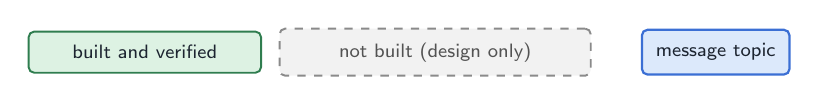
\begin{tikzpicture}[baseline]
    \node[ok,text width=2.6cm,font=\scriptsize] (a) {built and verified};
    \node[todo,text width=3.6cm,font=\scriptsize,right=6pt of a] {not built (design only)};
    \node[topic,right=6pt of a,xshift=4.6cm,font=\scriptsize\sffamily] {message topic};
  \end{tikzpicture}}

\begin{document}

%% ============================================================ PAGE 1
\pagetitle{1. The six layers at a glance}{Recurrent concept drift detection and model recall in a data stream via concept fingerprinting and pattern matching}
\legend\par\vspace{10pt}

\begin{center}
\begin{adjustbox}{max width=\textwidth,max height=0.74\textheight}
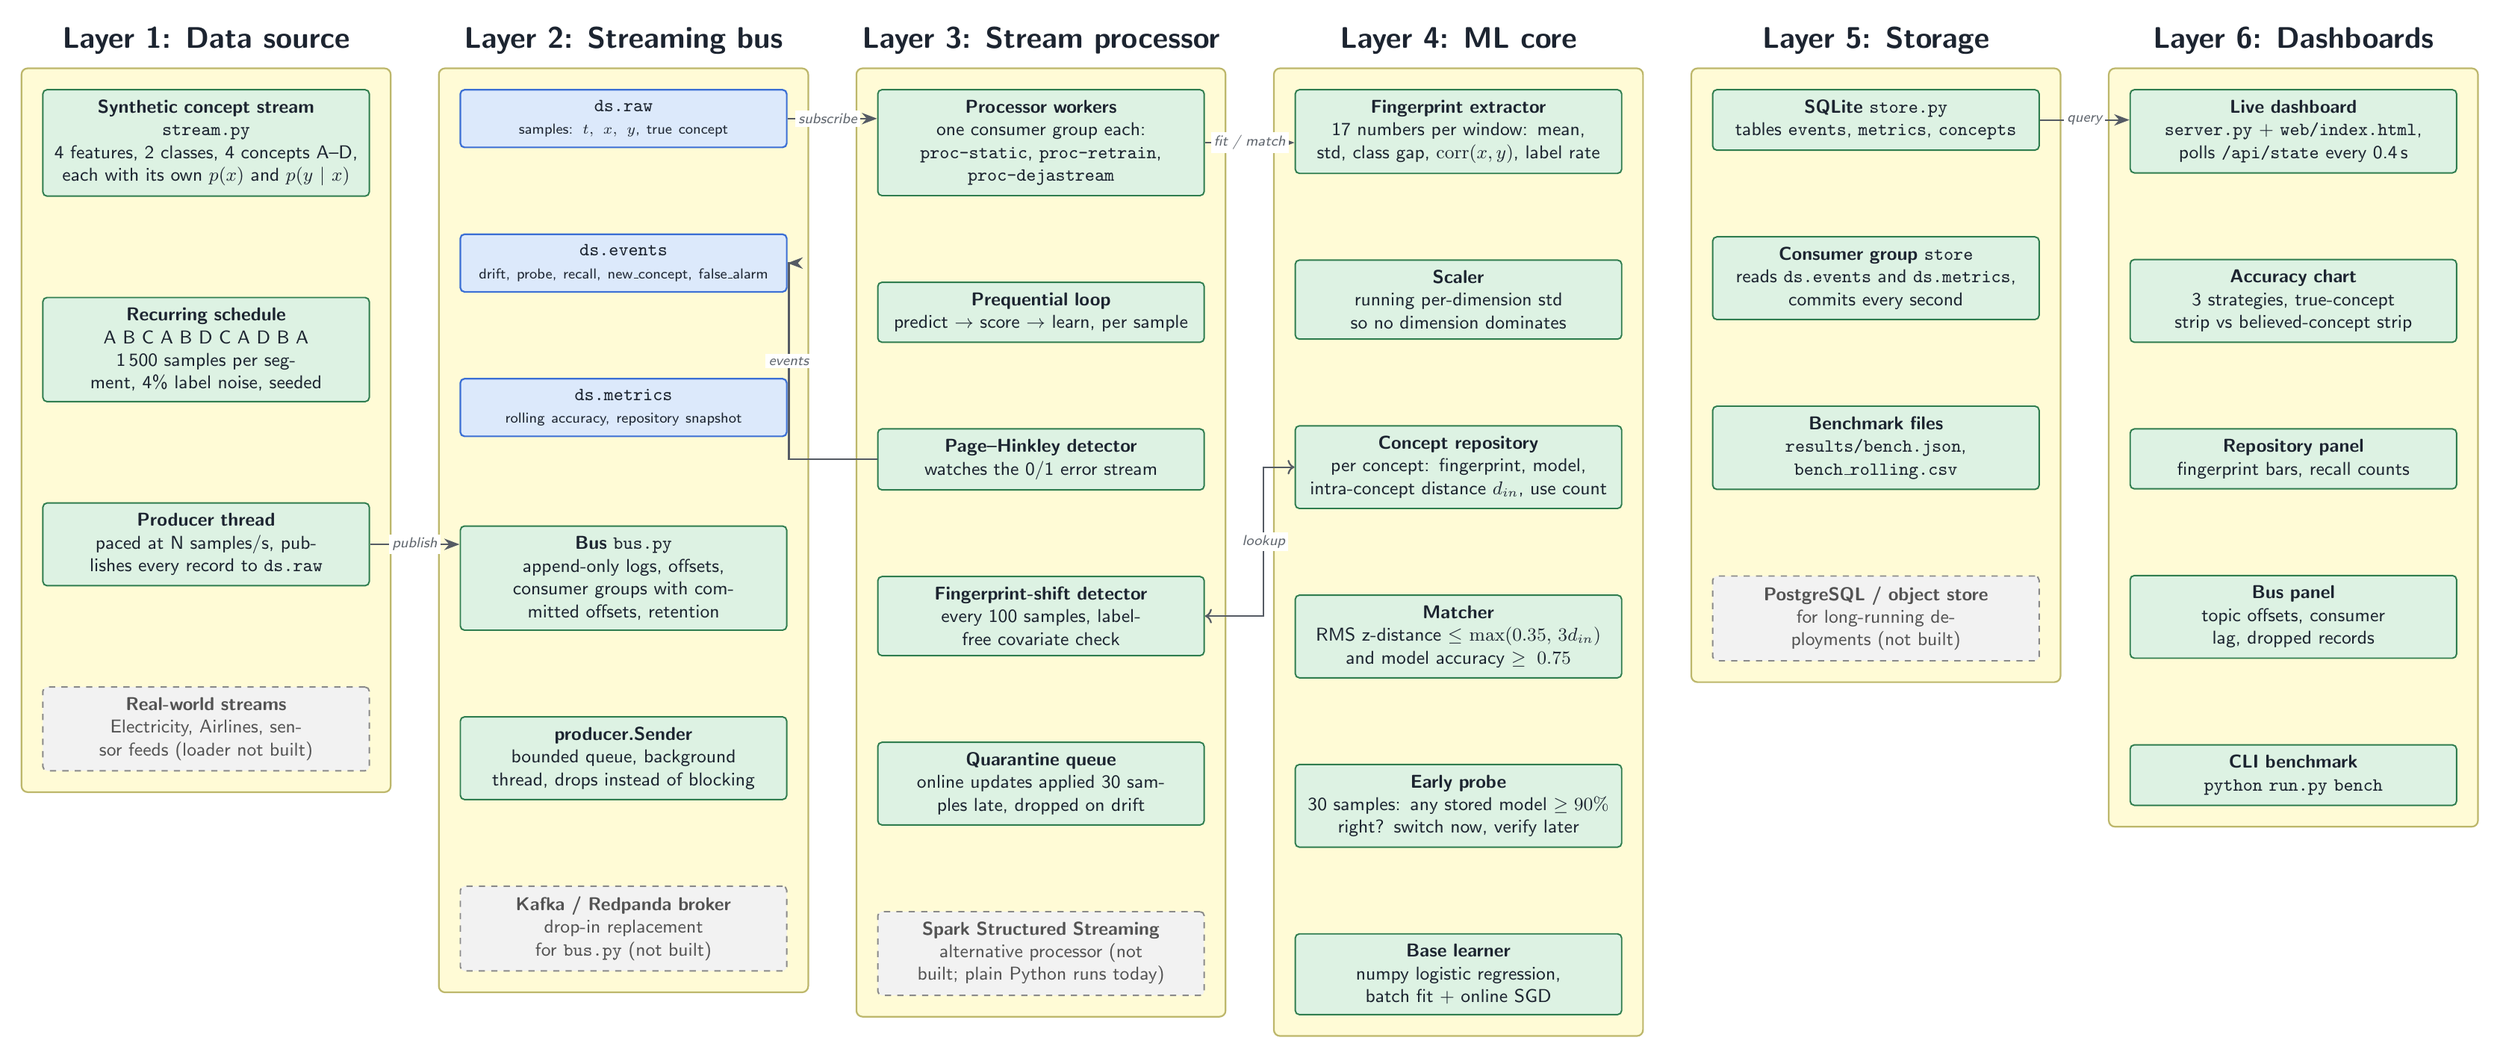
\begin{tikzpicture}[x=1cm,y=1cm]
  % column anchors
  \foreach \i/\x in {1/0,2/7.1,3/14.2,4/21.3,5/28.4,6/35.5}{\coordinate (c\i) at (\x,0);}

  % ---- layer 1
  \node[ok,anchor=north] (s1) at ($(c1)+(0,-1.4)$) {\textbf{Synthetic concept stream}\\\texttt{stream.py}\\4 features, 2 classes, 4 concepts A--D, each with its own $p(x)$ and $p(y\mid x)$};
  \node[ok,anchor=north] (s2) at ($(s1.south)+(0,-1.7)$) {\textbf{Recurring schedule}\\A B C A B D C A D B A\\1\,500 samples per segment, 4\% label noise, seeded};
  \node[ok,anchor=north] (s3) at ($(s2.south)+(0,-1.7)$) {\textbf{Producer thread}\\paced at N samples/s, publishes every record to \texttt{ds.raw}};
  \node[todo,anchor=north] (s4) at ($(s3.south)+(0,-1.7)$) {\textbf{Real-world streams}\\Electricity, Airlines, sensor feeds (loader not built)};

  % ---- layer 2
  \node[topic,anchor=north,text width=5.2cm] (t1) at ($(c2)+(0,-1.4)$) {ds.raw\\{\scriptsize\sffamily samples: $t,\ x,\ y$, true concept}};
  \node[topic,anchor=north,text width=5.2cm] (t2) at ($(t1.south)+(0,-1.45)$) {ds.events\\{\scriptsize\sffamily drift, probe, recall, new\_concept, false\_alarm}};
  \node[topic,anchor=north,text width=5.2cm] (t3) at ($(t2.south)+(0,-1.45)$) {ds.metrics\\{\scriptsize\sffamily rolling accuracy, repository snapshot}};
  \node[ok,anchor=north] (b1) at ($(t3.south)+(0,-1.5)$) {\textbf{Bus} \texttt{bus.py}\\append-only logs, offsets, consumer groups with committed offsets, retention};
  \node[ok,anchor=north] (b2) at ($(b1.south)+(0,-1.45)$) {\textbf{producer.Sender}\\bounded queue, background thread, drops instead of blocking};
  \node[todo,anchor=north] (b3) at ($(b2.south)+(0,-1.45)$) {\textbf{Kafka / Redpanda broker}\\drop-in replacement for \texttt{bus.py} (not built)};

  % ---- layer 3
  \node[ok,anchor=north] (p1) at ($(c3)+(0,-1.4)$) {\textbf{Processor workers}\\one consumer group each:\\\texttt{proc-static}, \texttt{proc-retrain}, \texttt{proc-dejastream}};
  \node[ok,anchor=north] (p2) at ($(p1.south)+(0,-1.45)$) {\textbf{Prequential loop}\\predict $\rightarrow$ score $\rightarrow$ learn, per sample};
  \node[ok,anchor=north] (p3) at ($(p2.south)+(0,-1.45)$) {\textbf{Page--Hinkley detector}\\watches the 0/1 error stream};
  \node[ok,anchor=north] (p4) at ($(p3.south)+(0,-1.45)$) {\textbf{Fingerprint-shift detector}\\every 100 samples, label-free covariate check};
  \node[ok,anchor=north] (p5) at ($(p4.south)+(0,-1.45)$) {\textbf{Quarantine queue}\\online updates applied 30 samples late, dropped on drift};
  \node[todo,anchor=north] (p6) at ($(p5.south)+(0,-1.45)$) {\textbf{Spark Structured Streaming}\\alternative processor (not built; plain Python runs today)};

  % ---- layer 4
  \node[ok,anchor=north] (m1) at ($(c4)+(0,-1.4)$) {\textbf{Fingerprint extractor}\\17 numbers per window: mean, std, class gap, $\mathrm{corr}(x,y)$, label rate};
  \node[ok,anchor=north] (m2) at ($(m1.south)+(0,-1.45)$) {\textbf{Scaler}\\running per-dimension std so no dimension dominates};
  \node[ok,anchor=north] (m3) at ($(m2.south)+(0,-1.45)$) {\textbf{Concept repository}\\per concept: fingerprint, model, intra-concept distance $d_{in}$, use count};
  \node[ok,anchor=north] (m4) at ($(m3.south)+(0,-1.45)$) {\textbf{Matcher}\\RMS z-distance $\le \max(0.35,\,3 d_{in})$ and model accuracy $\ge 0.75$};
  \node[ok,anchor=north] (m5) at ($(m4.south)+(0,-1.45)$) {\textbf{Early probe}\\30 samples: any stored model $\ge 90\%$ right? switch now, verify later};
  \node[ok,anchor=north] (m6) at ($(m5.south)+(0,-1.45)$) {\textbf{Base learner}\\numpy logistic regression, batch fit + online SGD};

  % ---- layer 5
  \node[ok,anchor=north] (d1) at ($(c5)+(0,-1.4)$) {\textbf{SQLite} \texttt{store.py}\\tables \texttt{events}, \texttt{metrics}, \texttt{concepts}};
  \node[ok,anchor=north] (d2) at ($(d1.south)+(0,-1.45)$) {\textbf{Consumer group \texttt{store}}\\reads \texttt{ds.events} and \texttt{ds.metrics}, commits every second};
  \node[ok,anchor=north] (d3) at ($(d2.south)+(0,-1.45)$) {\textbf{Benchmark files}\\\texttt{results/bench.json}, \texttt{bench\_rolling.csv}};
  \node[todo,anchor=north] (d4) at ($(d3.south)+(0,-1.45)$) {\textbf{PostgreSQL / object store}\\for long-running deployments (not built)};

  % ---- layer 6
  \node[ok,anchor=north] (v1) at ($(c6)+(0,-1.4)$) {\textbf{Live dashboard}\\\texttt{server.py} + \texttt{web/index.html}, polls \texttt{/api/state} every 0.4\,s};
  \node[ok,anchor=north] (v2) at ($(v1.south)+(0,-1.45)$) {\textbf{Accuracy chart}\\3 strategies, true-concept strip vs believed-concept strip};
  \node[ok,anchor=north] (v3) at ($(v2.south)+(0,-1.45)$) {\textbf{Repository panel}\\fingerprint bars, recall counts};
  \node[ok,anchor=north] (v4) at ($(v3.south)+(0,-1.45)$) {\textbf{Bus panel}\\topic offsets, consumer lag, dropped records};
  \node[ok,anchor=north] (v5) at ($(v4.south)+(0,-1.45)$) {\textbf{CLI benchmark}\\\texttt{python run.py bench}};

  % layer backgrounds
  \begin{scope}[on background layer]
    \node[layer,fit=(s1)(s4)] (L1) {};
    \node[layer,fit=(t1)(b3)] (L2) {};
    \node[layer,fit=(p1)(p6)] (L3) {};
    \node[layer,fit=(m1)(m6)] (L4) {};
    \node[layer,fit=(d1)(d4)] (L5) {};
    \node[layer,fit=(v1)(v5)] (L6) {};
  \end{scope}
  \foreach \i/\n in {1/{Layer 1: Data source},2/{Layer 2: Streaming bus},3/{Layer 3: Stream processor},4/{Layer 4: ML core},5/{Layer 5: Storage},6/{Layer 6: Dashboards}}{
    \node[title,anchor=south] at ($(L\i.north)+(0,3pt)$) {\n};}

  % flows between layers
  \draw[flow] (s3.east) -- node[lbl,pos=.5] {publish} (t1.west |- s3.east);
  \draw[flow] (t1.east) -- node[lbl,pos=.45] {subscribe} (p1.west |- t1.east);
  \draw[flow] (p3.west) -- ++(-1.5,0) |- node[lbl,pos=.25] {events} (t2.east);
  \draw[flow] (p1.east) -- node[lbl] {fit / match} (m1.west |- p1.east);
  \draw[flow,<->] (p4.east) -- ++(1.0,0) |- node[lbl,pos=.25] {lookup} (m3.west);
  \draw[flow] (d1.east) -- node[lbl] {query} (v1.west |- d1.east);
\end{tikzpicture}
\end{adjustbox}
\end{center}

\vfill
{\footnotesize\color{ink!70}
\textbf{Reading the diagram.} Publishers never talk to the processor and the processor never talks to the dashboard. Each side only knows the bus (or the database), so any part can restart or run at a different speed without losing events. Solid green boxes exist in this repository and are exercised by the tests; dashed grey boxes are the planned production swap-ins.}
\clearpage

%% ============================================================ PAGE 2
\pagetitle{2. Publish / subscribe in detail}{Topics are append-only logs. Every consumer group keeps its own committed offset, so each reader runs at its own speed.}

\begin{center}
\begin{adjustbox}{max width=\textwidth,max height=0.74\textheight}
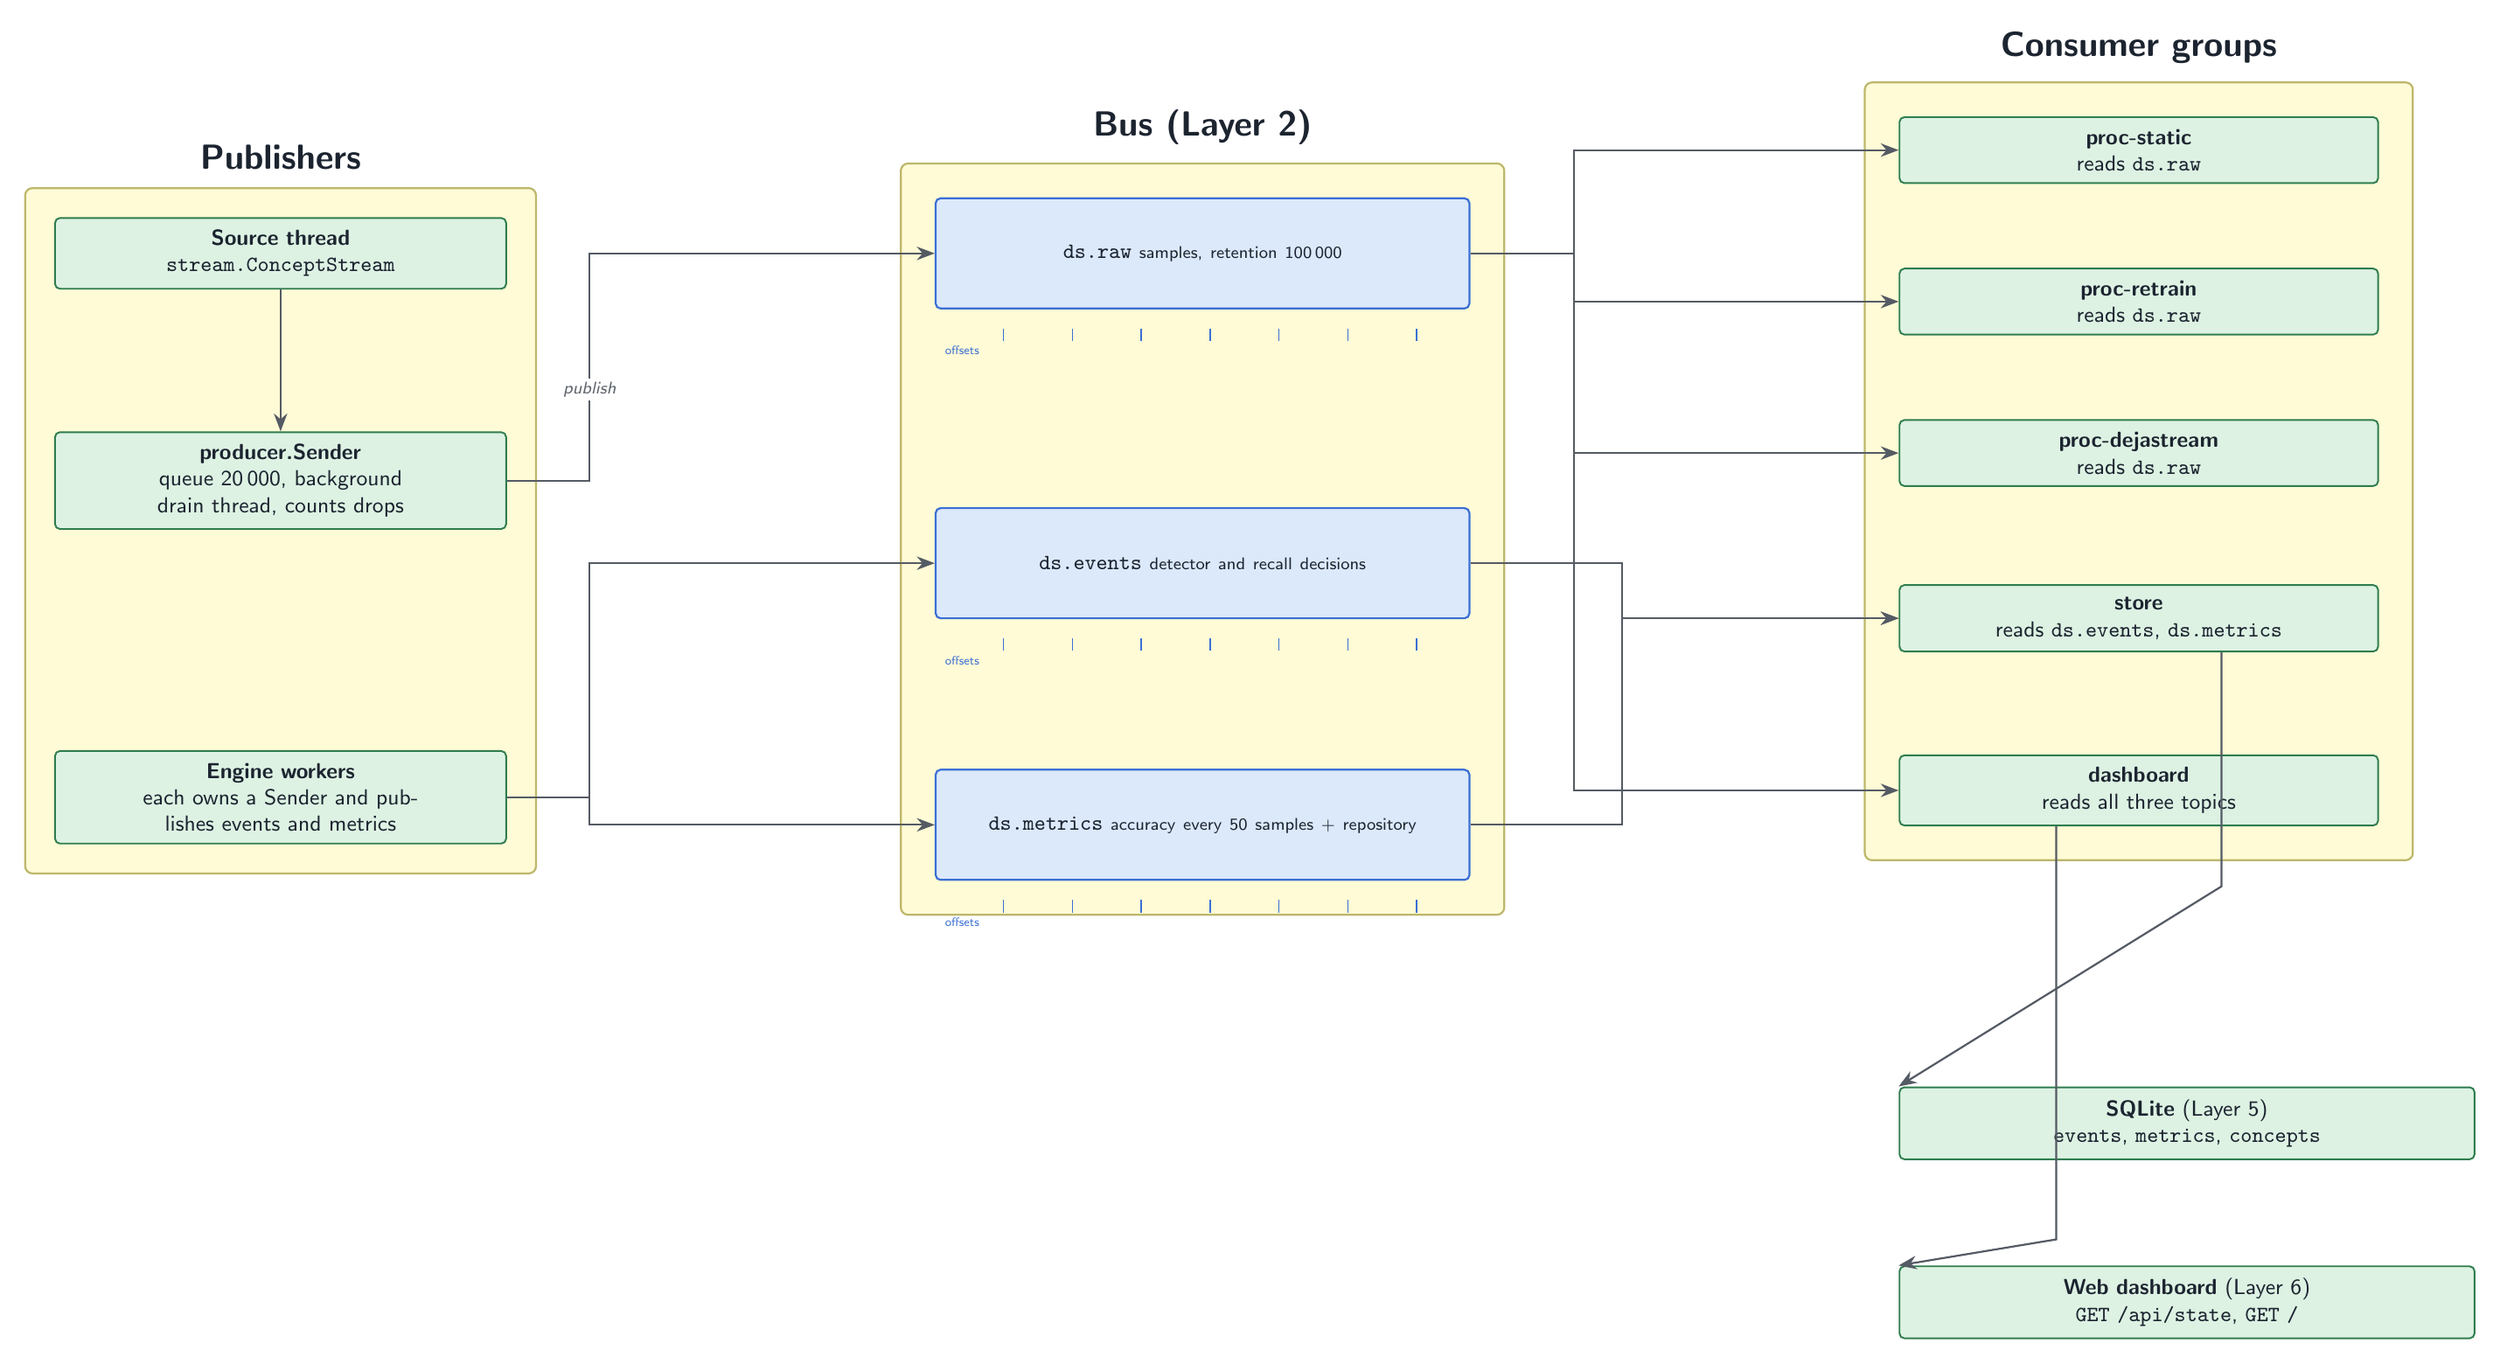
\begin{tikzpicture}[x=1cm,y=1cm]
  % producers
  \node[ok,text width=6.2cm] (src) at (0,5.5) {\textbf{Source thread}\\\texttt{stream.ConceptStream}};
  \node[ok,text width=6.2cm] (snd1) at (0,2.2) {\textbf{producer.Sender}\\queue 20\,000, background drain thread, counts drops};
  \node[ok,text width=6.2cm] (pe) at (0,-2.4) {\textbf{Engine workers}\\each owns a Sender and publishes events and metrics};
  \begin{scope}[on background layer]
    \node[layer,fit=(src)(snd1)(pe),inner sep=12pt] (PUB) {};
  \end{scope}
  \node[title,anchor=south] at ($(PUB.north)+(0,4pt)$) {Publishers};
  \draw[flow] (src) -- (snd1);

  % topics
  \node[topic,text width=7.4cm,minimum height=1.6cm,anchor=west] (tr) at (9.5,5.5) {ds.raw  {\scriptsize\sffamily samples, retention 100\,000}};
  \node[topic,text width=7.4cm,minimum height=1.6cm,anchor=west] (te) at (9.5,1.0) {ds.events  {\scriptsize\sffamily detector and recall decisions}};
  \node[topic,text width=7.4cm,minimum height=1.6cm,anchor=west] (tm) at (9.5,-2.8) {ds.metrics  {\scriptsize\sffamily accuracy every 50 samples + repository}};
  % offset ticks
  \foreach \t/\y in {tr/5.5,te/1.0,tm/-2.8}{
    \foreach \k in {0,...,6}{\draw[busline,line width=.5pt] ($(\t.south west)+(1.0+\k*1.0,-0.28)$) -- ++(0,-.18);}
    \node[font=\tiny,text=busline] at ($(\t.south west)+(0.4,-0.6)$) {offsets};
  }
  \begin{scope}[on background layer]
    \node[layer,fit=(tr)(te)(tm),inner sep=14pt] (BUS) {};
  \end{scope}
  \node[title,anchor=south] at ($(BUS.north)+(0,4pt)$) {Bus (Layer 2)};

  \draw[flow] (snd1.east) -- ++(1.2,0) |- node[lbl,pos=.2] {publish} (tr.west);
  \draw[flow] (pe.east) -- ++(1.2,0) |- (te.west);
  \draw[flow] (pe.east) -- ++(1.2,0) |- (tm.west);

  % consumer groups
  \node[ok,text width=6.6cm,anchor=west] (g1) at (23.5,7.0) {\textbf{proc-static}\\reads \texttt{ds.raw}};
  \node[ok,text width=6.6cm,anchor=west] (g2) at (23.5,4.8) {\textbf{proc-retrain}\\reads \texttt{ds.raw}};
  \node[ok,text width=6.6cm,anchor=west] (g3) at (23.5,2.6) {\textbf{proc-dejastream}\\reads \texttt{ds.raw}};
  \node[ok,text width=6.6cm,anchor=west] (g4) at (23.5,0.2) {\textbf{store}\\reads \texttt{ds.events}, \texttt{ds.metrics}};
  \node[ok,text width=6.6cm,anchor=west] (g5) at (23.5,-2.3) {\textbf{dashboard}\\reads all three topics};
  \begin{scope}[on background layer]
    \node[layer,fit=(g1)(g5),inner sep=14pt] (CG) {};
  \end{scope}
  \node[title,anchor=south] at ($(CG.north)+(0,4pt)$) {Consumer groups};

  \foreach \g in {g1,g2,g3}{\draw[flow] (tr.east) -- ++(1.5,0) |- (\g.west);}
  \draw[flow] (te.east) -- ++(2.2,0) |- (g4.west);
  \draw[flow] (tm.east) -- ++(2.2,0) |- (g4.west);
  \draw[flow] (tr.east) -- ++(1.5,0) |- (g5.west);

  % consumers outputs
  \node[ok,text width=8cm,anchor=north west] (sq) at (23.5,-6.6) {\textbf{SQLite} (Layer 5)\\\texttt{events}, \texttt{metrics}, \texttt{concepts}};
  \node[ok,text width=8cm,anchor=north west] (web) at (23.5,-9.2) {\textbf{Web dashboard} (Layer 6)\\\texttt{GET /api/state}, \texttt{GET /}};
  \draw[flow] (g4.south) ++(1.2,0) -- ++(0,-3.4) -- (sq.north west |- sq.north);
  \draw[flow] (g5.south) ++(-1.2,0) -- ++(0,-6.0) -- (web.north west |- web.north);
\end{tikzpicture}
\end{adjustbox}
\end{center}

\vspace{2pt}
\begin{tabular}{@{}p{12cm}p{12cm}p{12cm}@{}}
\textbf{Why a bus at all?} The three strategies read the \emph{same} \texttt{ds.raw} log independently, so the comparison is fair and they never block each other. &
\textbf{Loss boundary.} The Sender queue is bounded: when full it drops and counts the record (\texttt{dropped} on the dashboard) rather than slowing the source. &
\textbf{Stand-in for Kafka.} \texttt{bus.py} implements topics, offsets, groups and lag in-process. A Kafka client can replace it without touching the engine.
\end{tabular}
\clearpage

%% ============================================================ PAGE 3
\pagetitle{3. Drift handling state machine}{\texttt{engine.py}: what one DejaStream engine does for every incoming sample}

\begin{center}
\begin{adjustbox}{max width=\textwidth,max height=0.74\textheight}
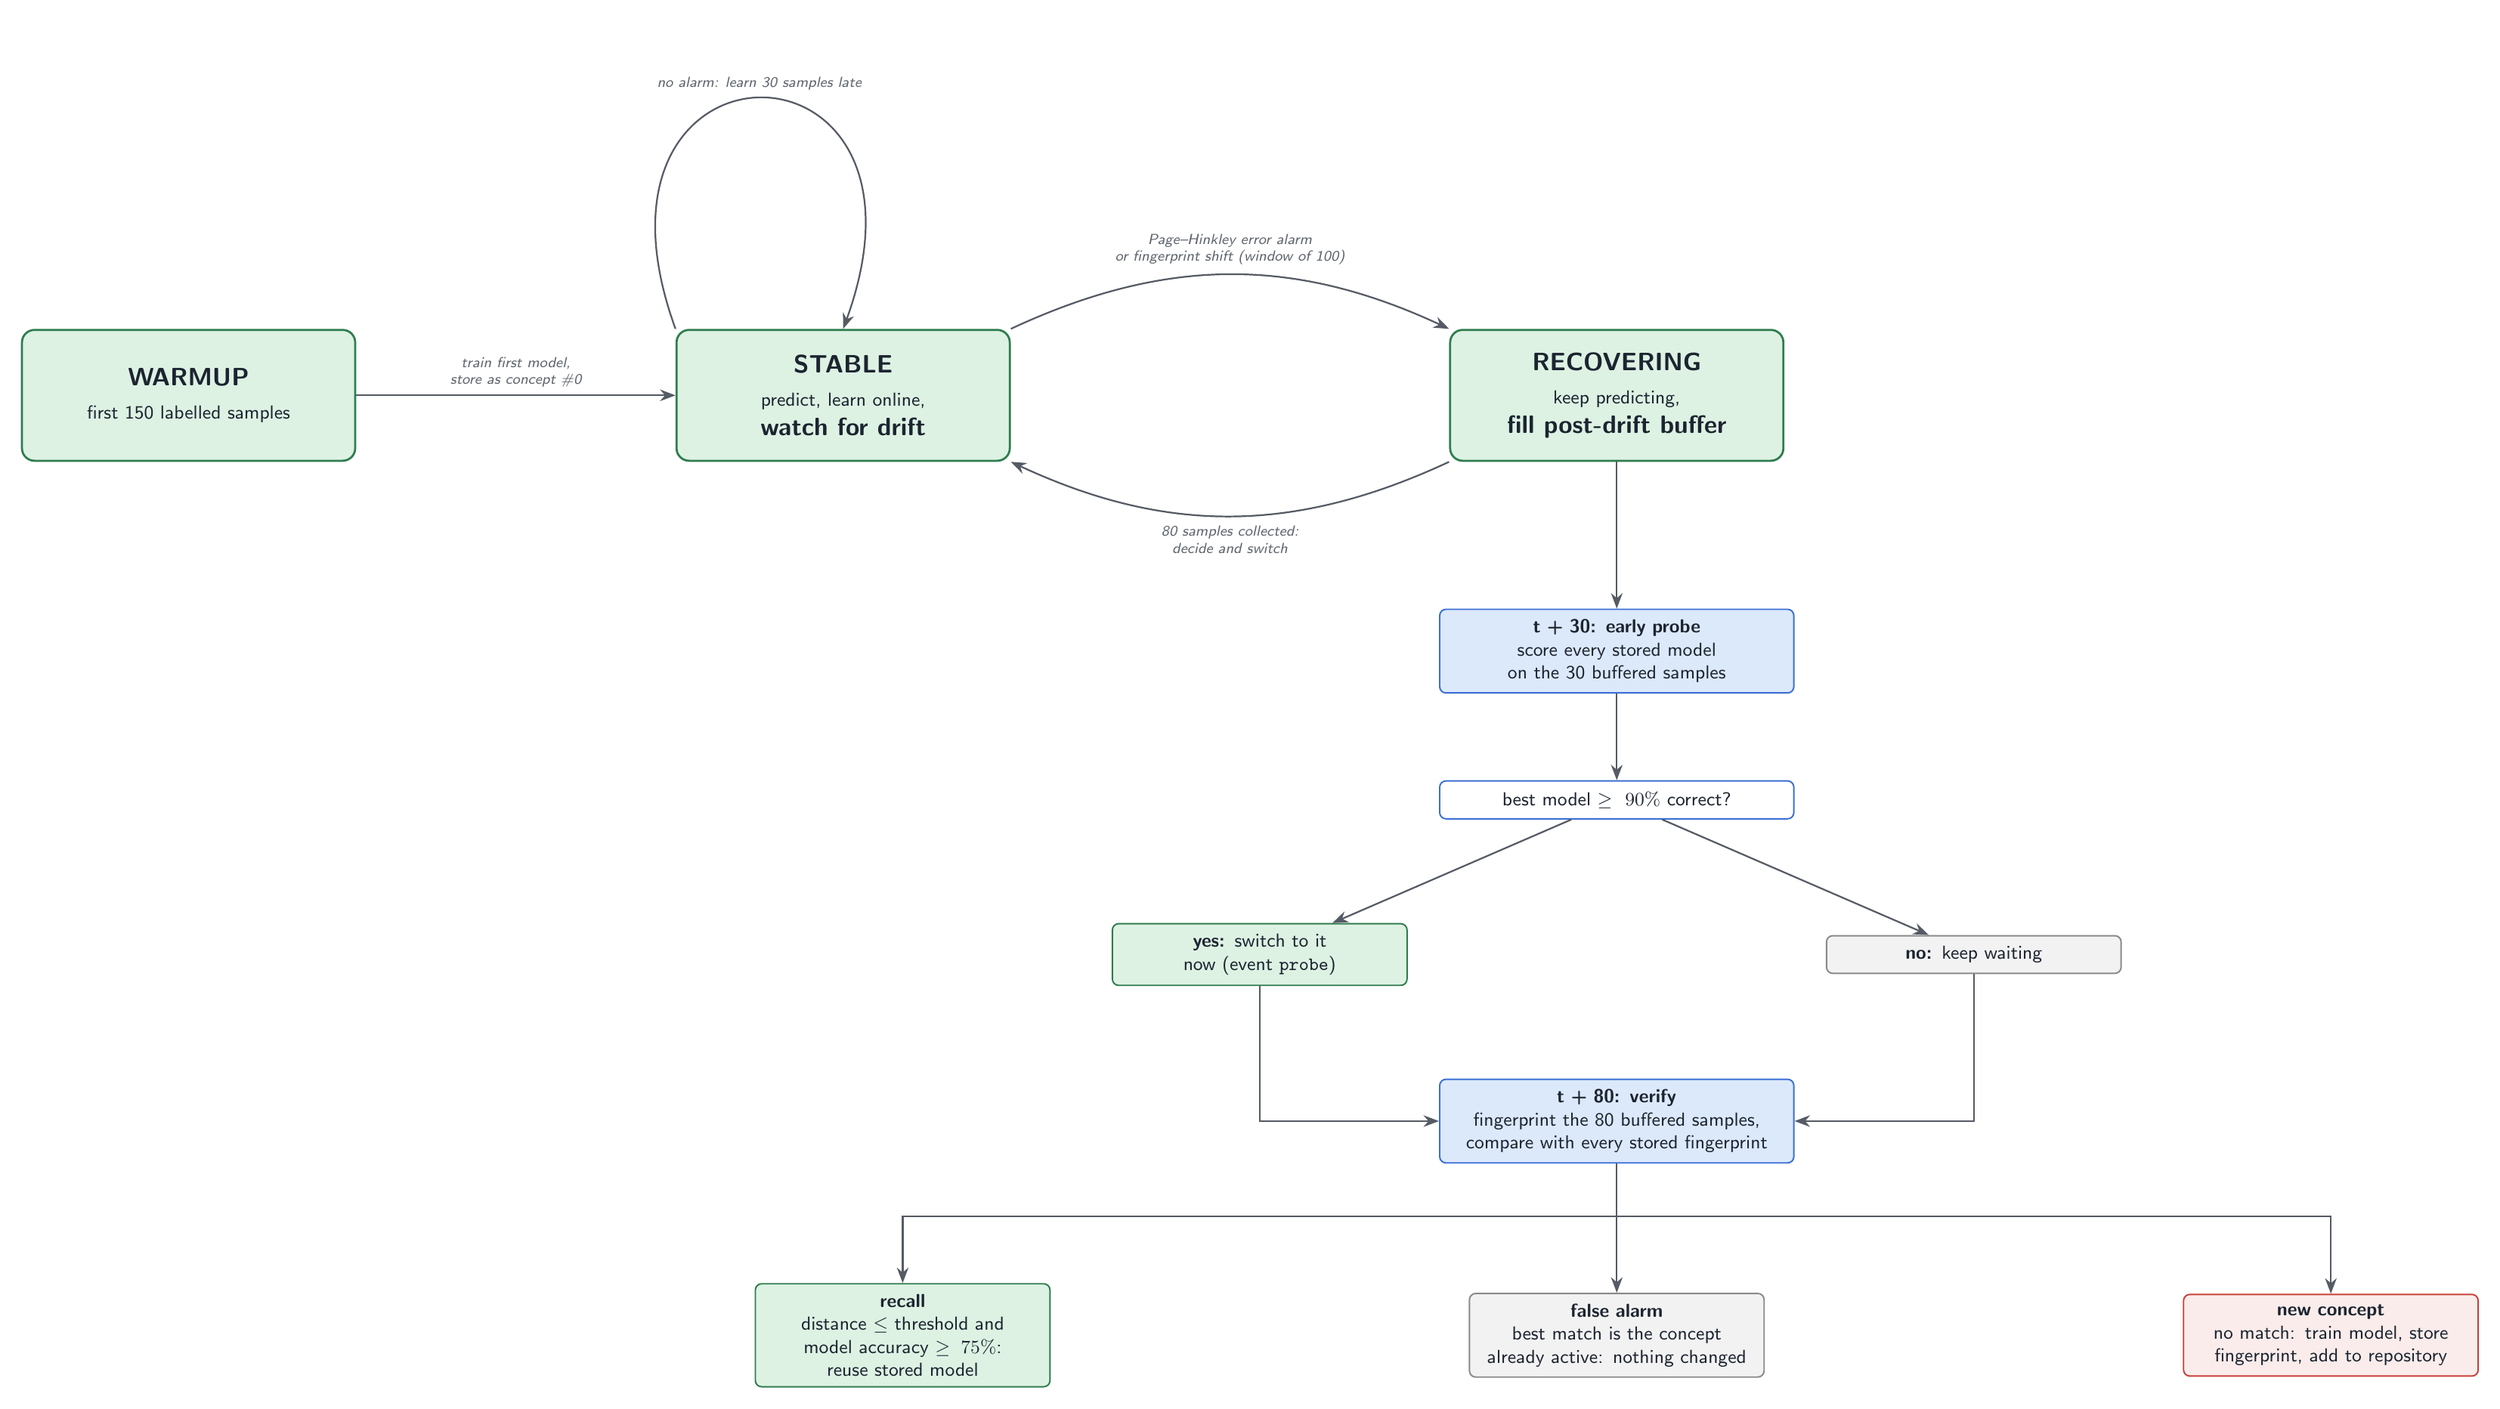
\begin{tikzpicture}[x=1cm,y=1cm,
  st/.style={draw=okline,fill=okfill,rounded corners=6pt,minimum width=5.6cm,minimum height=2.2cm,align=center,font=\large\bfseries,line width=1pt,text=ink},
  stp/.style={draw=busline,fill=busfill,rounded corners=3pt,align=center,text width=5.6cm,inner sep=5pt,font=\small,text=ink,line width=.7pt},
  outc/.style={draw=okline,fill=okfill,rounded corners=3pt,align=center,text width=4.6cm,inner sep=5pt,font=\small,text=ink,line width=.7pt}]
  \node[st] (warm) at (0,0) {WARMUP\\[2pt]\normalfont\small first 150 labelled samples};
  \node[st] (stab) at (11,0) {STABLE\\[2pt]\normalfont\small predict, learn online,\\watch for drift};
  \node[st] (rec) at (24,0) {RECOVERING\\[2pt]\normalfont\small keep predicting,\\fill post-drift buffer};

  \draw[flow] (warm) -- node[lbl,above=2pt,text width=3.2cm,align=center] {train first model,\\store as concept \#0} (stab);
  \draw[flow] (stab.north east) to[bend left=25] node[lbl,above=3pt,text width=6.2cm,align=center] {Page--Hinkley error alarm\\or fingerprint shift (window of 100)} (rec.north west);
  \draw[flow] (rec.south west) to[bend left=25] node[lbl,below=3pt,text width=5cm,align=center] {80 samples collected:\\decide and switch} (stab.south east);
  \draw[flow,looseness=6] (stab.north west) to[out=110,in=70,looseness=5] node[lbl,above=2pt,pos=.5] {no alarm: learn 30 samples late} (stab.north);

  % recovery detail
  \node[stp] (a) at (24,-4.3) {\textbf{t + 30: early probe}\\score every stored model on the 30 buffered samples};
  \node[stp,fill=white] (b) at (24,-6.8) {best model $\ge 90\%$ correct?};
  \node[outc] (p1) at (18,-9.4) {\textbf{yes:} switch to it now (event \texttt{probe})};
  \node[outc,draw=todoline,fill=todofill] (p2) at (30,-9.4) {\textbf{no:} keep waiting};
  \node[stp] (c) at (24,-12.2) {\textbf{t + 80: verify}\\fingerprint the 80 buffered samples, compare with every stored fingerprint};
  \node[outc] (o1) at (12,-15.8) {\textbf{recall}\\distance $\le$ threshold and model accuracy $\ge 75\%$: reuse stored model};
  \node[outc,draw=todoline,fill=todofill] (o2) at (24,-15.8) {\textbf{false alarm}\\best match is the concept already active: nothing changed};
  \node[outc,draw=bad,fill=bad!10] (o3) at (36,-15.8) {\textbf{new concept}\\no match: train model, store fingerprint, add to repository};

  \draw[flow] (rec) -- (a);
  \draw[flow] (a) -- (b);
  \draw[flow] (b) -- (p1); \draw[flow] (b) -- (p2);
  \draw[flow] (p1) |- (c); \draw[flow] (p2) |- (c);
  \draw[flow] (c) -- ++(0,-1.6) -| (o1); \draw[flow] (c) -- ++(0,-1.6) -| (o3); \draw[flow] (c) -- (o2);
\end{tikzpicture}
\end{adjustbox}
\end{center}
\vfill
{\footnotesize\color{ink!70}\textbf{Retrain baseline} uses the same Page--Hinkley detector but always trains a fresh model from its 80 buffered samples and keeps no memory. \textbf{Static baseline} trains once and never adapts. The quarantine queue (30 samples) keeps online learning from polluting a stored model during the roughly 13-sample detection delay.}
\clearpage

%% ============================================================ PAGE 4
\pagetitle{4. Concept fingerprinting and pattern matching}{\texttt{fingerprint.py}, \texttt{engine.\_match}: how a window of data becomes a recognisable signature}

\begin{center}
\begin{adjustbox}{max width=\textwidth,max height=0.74\textheight}
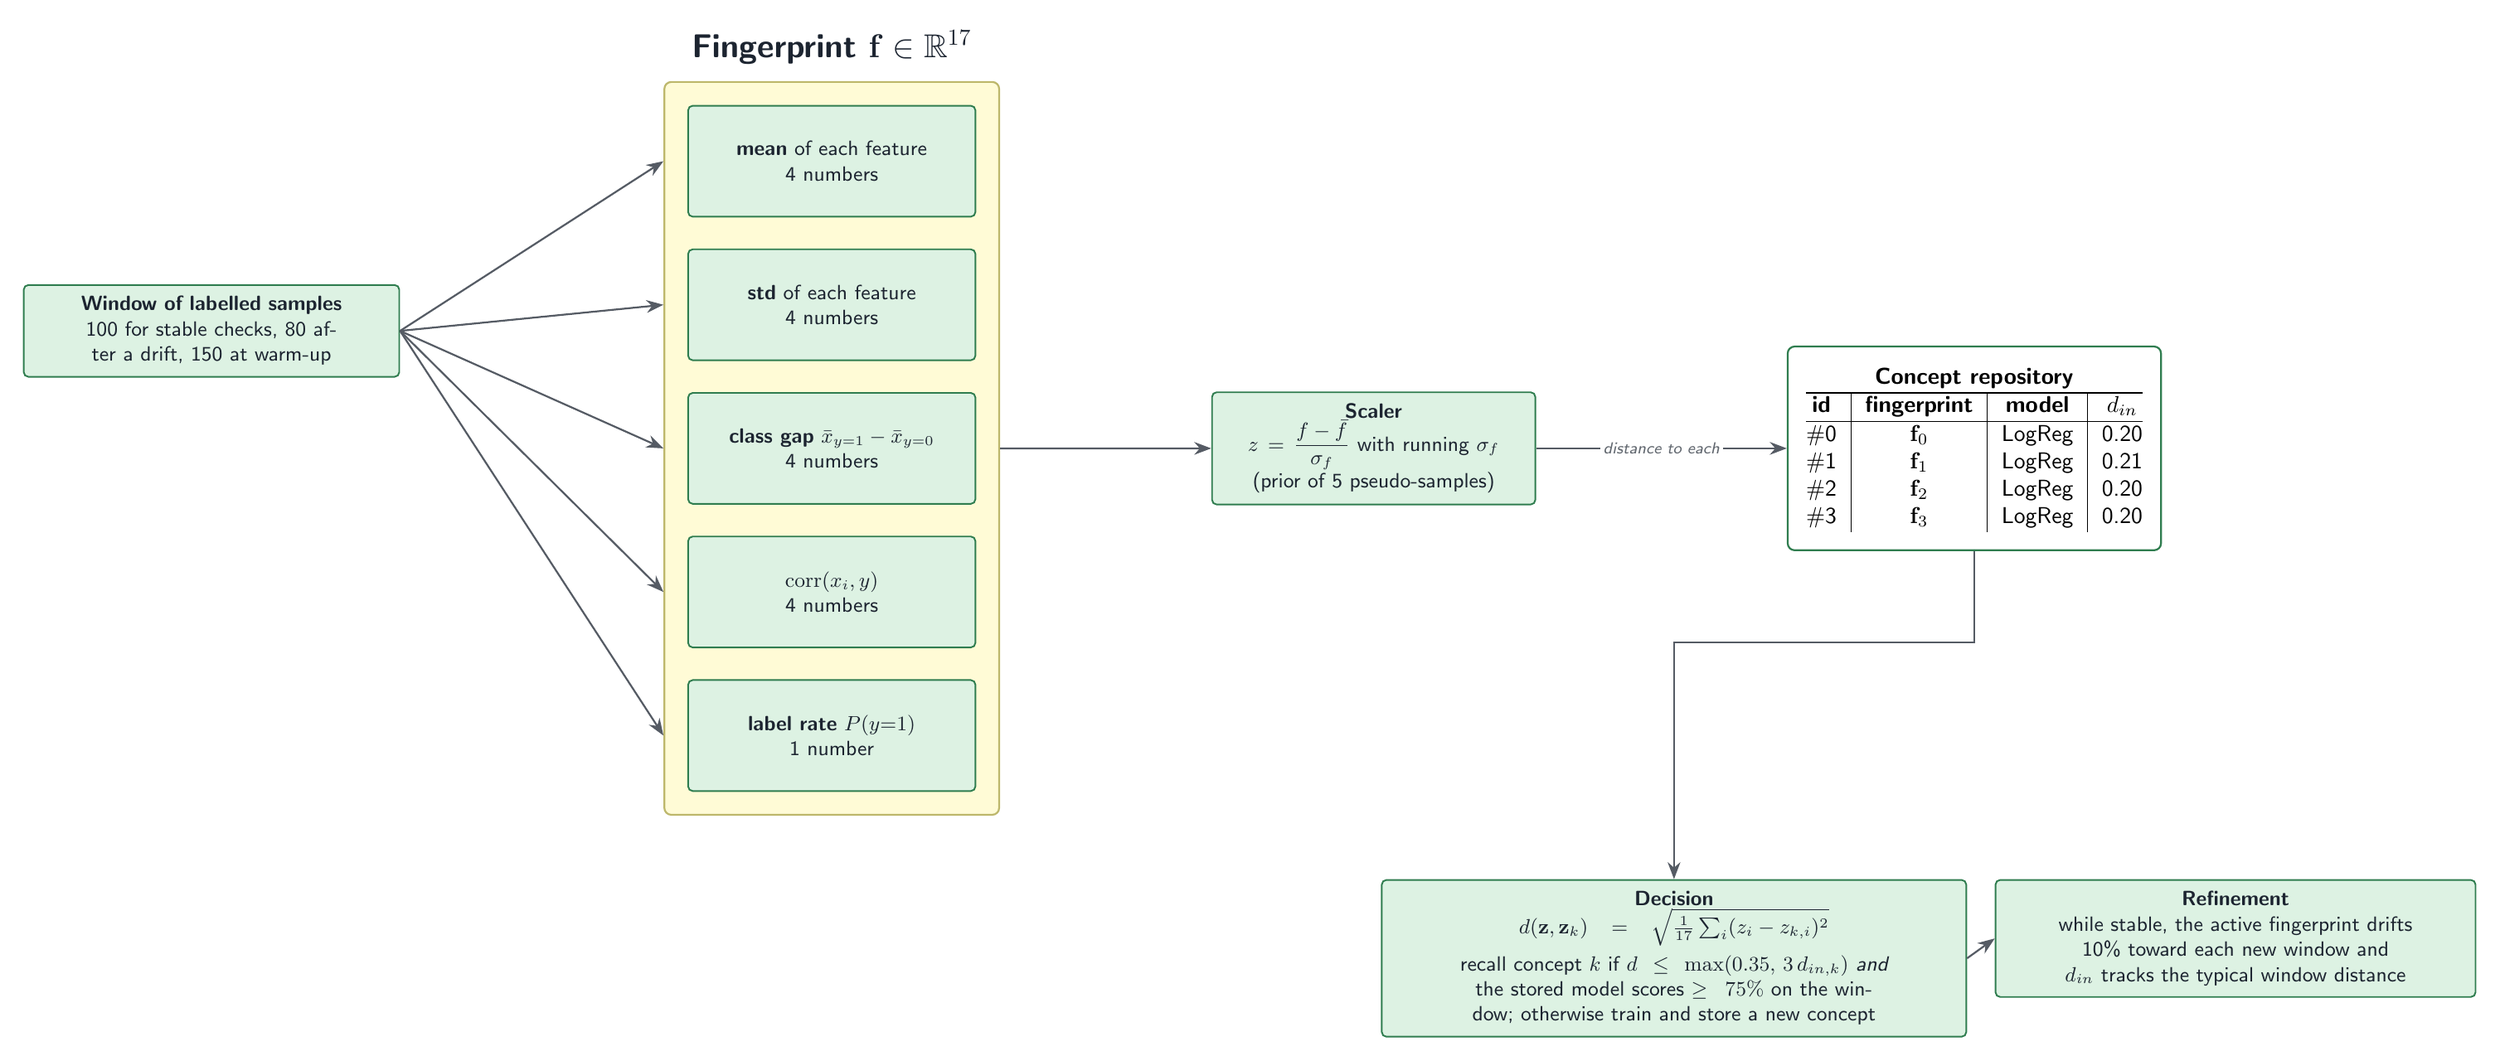
\begin{tikzpicture}[x=1cm,y=1cm,
  fp/.style={draw=okline,fill=okfill,rounded corners=2pt,minimum height=1.7cm,align=center,font=\small,text=ink,line width=.7pt}]
  \node[ok,text width=5.4cm] (win) at (0,0) {\textbf{Window of labelled samples}\\100 for stable checks, 80 after a drift, 150 at warm-up};

  % fingerprint vector
  \node[fp,minimum width=4.4cm] (f1) at (9.5,2.6) {\textbf{mean} of each feature\\4 numbers};
  \node[fp,minimum width=4.4cm] (f2) at (9.5,0.4) {\textbf{std} of each feature\\4 numbers};
  \node[fp,minimum width=4.4cm] (f3) at (9.5,-1.8) {\textbf{class gap} $\bar x_{y=1}-\bar x_{y=0}$\\4 numbers};
  \node[fp,minimum width=4.4cm] (f4) at (9.5,-4.0) {$\mathrm{corr}(x_i,y)$\\4 numbers};
  \node[fp,minimum width=4.4cm] (f5) at (9.5,-6.2) {\textbf{label rate} $P(y{=}1)$\\1 number};
  \begin{scope}[on background layer]\node[layer,fit=(f1)(f5)] (FP) {};\end{scope}
  \node[title,anchor=south] at ($(FP.north)+(0,4pt)$) {Fingerprint $\mathbf f\in\mathbb R^{17}$};
  \foreach \f in {f1,f2,f3,f4,f5}{\draw[flow] (win.east) -- ($(FP.west |- \f.west)$);}

  \node[ok,text width=4.6cm] (sc) at (17.8,-1.8) {\textbf{Scaler}\\$z=\dfrac{f-\bar f}{\sigma_f}$ with running $\sigma_f$ (prior of 5 pseudo-samples)};
  \draw[flow] (FP.east) -- (sc.west);

  % repository
  \node[draw=okline,fill=white,rounded corners=3pt,line width=.8pt,inner sep=8pt] (repo) at (27,-1.8) {%
  \begin{tabular}{@{}c|c|c|c@{}}
    \multicolumn{4}{c}{\textbf{Concept repository}}\\\hline
    \textbf{id} & \textbf{fingerprint} & \textbf{model} & \textbf{$d_{in}$}\\\hline
    \#0 & $\mathbf f_0$ & LogReg & 0.20\\
    \#1 & $\mathbf f_1$ & LogReg & 0.21\\
    \#2 & $\mathbf f_2$ & LogReg & 0.20\\
    \#3 & $\mathbf f_3$ & LogReg & 0.20\\
  \end{tabular}};
  \draw[flow] (sc.east) -- node[lbl] {distance to each} (repo.west);

  \node[ok,text width=8.6cm,anchor=north] (rule) at (22.4,-8.4) {\textbf{Decision}\\$d(\mathbf z,\mathbf z_k)=\sqrt{\tfrac1{17}\sum_i (z_i-z_{k,i})^2}$\\[3pt]
  recall concept $k$ if $d\le\max(0.35,\,3\,d_{in,k})$ \emph{and} the stored model scores $\ge75\%$ on the window; otherwise train and store a new concept};
  \draw[flow] (repo.south) -- ++(0,-1.4) -| (rule.north);

  \node[ok,text width=7cm,anchor=north] (upd) at (31,-8.4) {\textbf{Refinement}\\while stable, the active fingerprint drifts 10\% toward each new window and $d_{in}$ tracks the typical window distance};
  \draw[flow] (rule.east) -- (upd.west);
\end{tikzpicture}
\end{adjustbox}
\end{center}
\vfill
\begin{tabular}{@{}p{12cm}p{12cm}p{12cm}@{}}
\textbf{Why four kinds of statistic?} Means and spreads see changes in $p(x)$. Class gaps and correlations see changes in how features relate to the label, which is what a plain error counter cannot localise. &
\textbf{Why scale?} Raw dimensions differ by orders of magnitude (label rate lives in $[0,1]$, means in $[-3,3]$). Z-scoring makes one threshold meaningful for all of them. &
\textbf{Two safeguards.} Intra-concept distance $d_{in}$ adapts the threshold to how noisy each concept is. The model-accuracy check stops two concepts with similar inputs but different labelling rules from being merged.
\end{tabular}
\clearpage

%% ============================================================ PAGE 5
\pagetitle{5. Measured behaviour}{\nsamples{} samples, \nchanges{} true concept changes, identical stream for all three strategies (\texttt{python run.py bench})}

\begin{center}
\begin{tikzpicture}
\begin{axis}[width=36cm,height=11.5cm,xlabel={sample index $t$},ylabel={rolling accuracy (100 samples)},ymin=0.1,ymax=1.02,xmin=0,xmax=16500,xtick distance=1500,scaled x ticks=false,
  grid=major,grid style={draw=ink!12},legend style={at={(0.5,1.07)},anchor=south,draw=none,legend columns=3,font=\normalsize},
  tick label style={font=\small},label style={font=\normalsize},every axis plot/.append style={line width=1.1pt}]
  % concept boundaries
  \pgfplotsinvokeforeach{1500,3000,4500,6000,7500,9000,10500,12000,13500,15000}{\draw[bad!50,dashed] (axis cs:#1,0.1) -- (axis cs:#1,1.02);}
  \addplot[cstatic] table[col sep=comma,x=t,y=static] {../results/bench_rolling.csv};
  \addplot[cretrain] table[col sep=comma,x=t,y=retrain] {../results/bench_rolling.csv};
  \addplot[cdeja,line width=1.5pt] table[col sep=comma,x=t,y=dejastream] {../results/bench_rolling.csv};
  \legend{static model,retrain on drift,DejaStream}
  \node[font=\small\bfseries,text=bad!80!black] at (axis cs:750,0.13) {A}; \node[font=\small\bfseries,text=bad!80!black] at (axis cs:2250,0.13) {B}; \node[font=\small\bfseries,text=bad!80!black] at (axis cs:3750,0.13) {C}; \node[font=\small\bfseries,text=bad!80!black] at (axis cs:5250,0.13) {A}; \node[font=\small\bfseries,text=bad!80!black] at (axis cs:6750,0.13) {B}; \node[font=\small\bfseries,text=bad!80!black] at (axis cs:8250,0.13) {D}; \node[font=\small\bfseries,text=bad!80!black] at (axis cs:9750,0.13) {C}; \node[font=\small\bfseries,text=bad!80!black] at (axis cs:11250,0.13) {A}; \node[font=\small\bfseries,text=bad!80!black] at (axis cs:12750,0.13) {D}; \node[font=\small\bfseries,text=bad!80!black] at (axis cs:14250,0.13) {B}; \node[font=\small\bfseries,text=bad!80!black] at (axis cs:15750,0.13) {A};
\end{axis}
\end{tikzpicture}
\end{center}

\vspace{4pt}
\begin{center}
\renewcommand{\arraystretch}{1.35}
\begin{tabular}{@{}lccccccc@{}}
\toprule
\textbf{Strategy} & \textbf{Overall acc.} & \textbf{Acc. first 300 after drift} & \textbf{Changes detected} & \textbf{Mean delay} & \textbf{Models trained} & \textbf{Recalls} & \textbf{False alarms}\\
\midrule
Static model & 58.7\% & 56.4\% & 0/10 & -- & 1 & 0 & 0 \\
Retrain on drift & 90.6\% & 76.7\% & 10/10 & 13.0 & 11 & 0 & 0 \\
DejaStream & 91.8\% & 83.2\% & 10/10 & 13.5 & 4 & 7 & 2 \\
\bottomrule
\end{tabular}

\end{center}
\vfill
{\footnotesize\color{ink!70}Red dashed lines mark the true concept changes; letters show the concept in force. Numbers are read from \texttt{results/bench.json} each time this PDF is built. Synthetic data, single seed: the result shows the mechanism works, not that it generalises to real streams. Detection delay is counted in samples after the true change.}
\clearpage

%% ============================================================ PAGE 6
\pagetitle{6. Code map}{Where each box in the diagrams lives in the repository}
\renewcommand{\arraystretch}{1.5}
\begin{tabular}{@{}p{6.2cm}p{2.2cm}p{20cm}p{3.6cm}@{}}
\toprule
\textbf{File} & \textbf{Layer} & \textbf{Responsibility} & \textbf{Status}\\
\midrule
\texttt{dejastream/stream.py} & 1 & Recurring-concept generator, segment schedule, label noise & \textcolor{okline}{built, tested}\\
\texttt{dejastream/bus.py} & 2 & Topics, offsets, consumer groups, retention, \texttt{Sender} with drop counting & \textcolor{okline}{built, tested}\\
\texttt{dejastream/pipeline.py} & 2--5 & Starts the source, one worker per strategy, the store and the dashboard consumers & \textcolor{okline}{built, run live}\\
\texttt{dejastream/detector.py} & 3 & Page--Hinkley drift detector on the error stream & \textcolor{okline}{built, tested}\\
\texttt{dejastream/engine.py} & 3--4 & State machine, quarantine, early probe, repository, matching, three strategies & \textcolor{okline}{built, tested}\\
\texttt{dejastream/fingerprint.py} & 4 & 17-d fingerprint and running scaler with RMS distance & \textcolor{okline}{built, tested}\\
\texttt{dejastream/models.py} & 4 & numpy logistic regression with batch fit and online SGD & \textcolor{okline}{built, tested}\\
\texttt{dejastream/store.py} & 5 & SQLite tables for events, metrics, concept snapshots & \textcolor{okline}{built, run live}\\
\texttt{dejastream/server.py}, \texttt{web/index.html} & 6 & HTTP server, canvas charts, repository, bus and event panels & \textcolor{okline}{built, run live}\\
\texttt{dejastream/bench.py}, \texttt{run.py} & 6 & Offline comparison, JSON and CSV export, CLI & \textcolor{okline}{built, tested}\\
\midrule
Kafka / Redpanda adapter & 2 & Replace \texttt{bus.py} with a real broker client & \textcolor{todoline}{not built}\\
Spark Structured Streaming processor & 3 & Alternative to the Python worker threads & \textcolor{todoline}{not built}\\
Real dataset loaders & 1 & Electricity, Airlines, sensor streams in place of the synthetic generator & \textcolor{todoline}{not built}\\
PostgreSQL storage & 5 & Production store in place of SQLite & \textcolor{todoline}{not built}\\
\bottomrule
\end{tabular}

\end{document}
